\section{El proceso de desarrollo}

Aproximadamente, la siguiente tabla (\ref{tab:proceso-dev}) recoge el tiempo
dedicado a cada una de las tareas llevadas a cabo durante el desarrollo del
proyecto.

\begin{table}[h]
\begin{center}
\begin{tabular}{lcl}
 \hline \hline
 \multicolumn{1}{c}{\textbf{Tarea}} &
 \multicolumn{1}{c}{\textbf{Fecha de comienzo}} &
 \multicolumn{1}{c}{\textbf{Tiempo \small{(d�as)}}} \\
 \hline \hline
 Estudio de viabilidad & 07/12/06 & 15\\
 \hline
 An�lisis y dise�o & 08/01/07 & 40\\
 \hline
 Desarrollo del software & 25/02/07 & 140\\
 \hline
 Elaboraci�n de la documentaci�n & 11/06/07 & 30\\
 \hline \hline
\end{tabular}
\caption{Tiempo de dedicaci�n a cada tarea}
\label{tab:proceso-dev}
\end{center}
\end{table}

En el gr�fico de la figura \ref{fig:svn-act} se muestra la actividad del
repositorio de c�digo y documentaci�n durante los �ltimos doce meses.

\begin{figure}[h]
\begin{center}
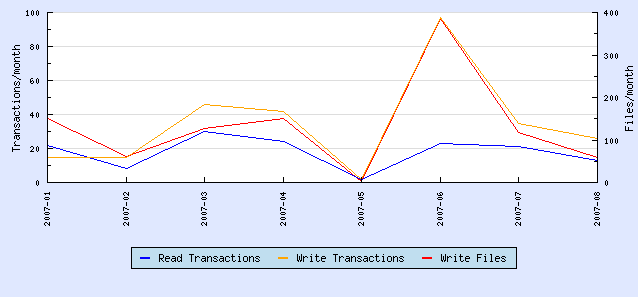
\includegraphics[scale=0.8]{images/svn-activity.png}
\end{center}
\caption[Gr�fico de actividad en el repositorio de c�digo y
documentaci�n]{Gr�fico de actividad en el repositorio SVN (SourceForge.net)}
\label{fig:svn-act}
\end{figure}